\begin{figure}
    \centering
    \begin{subfigure}{\textwidth}
        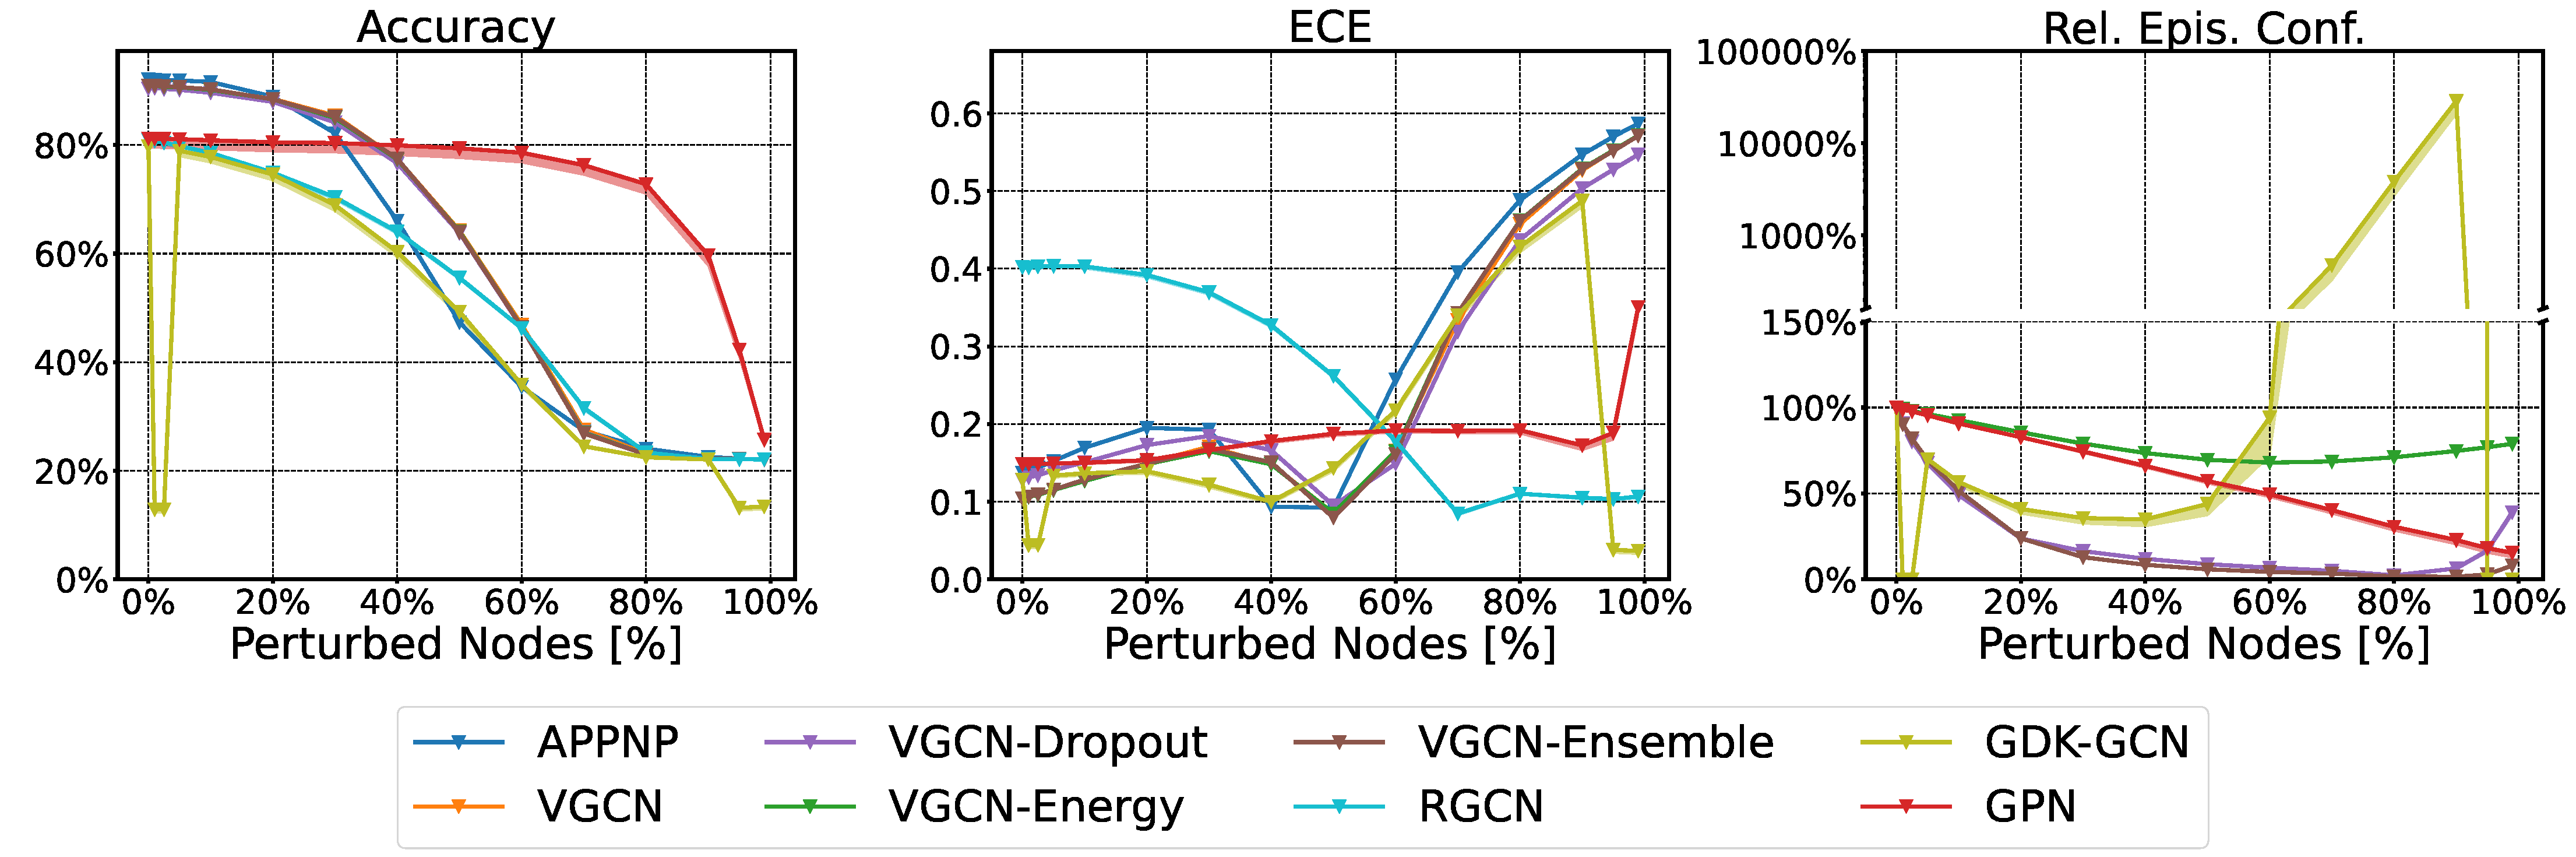
\includegraphics[width=\textwidth]{sections/009_neurips2021/resources/plots/AmazonPhotos-bernoulli-shift.pdf}
        \caption{Bernoulli Feature Shift}
    \end{subfigure}
    \begin{subfigure}{\textwidth}
        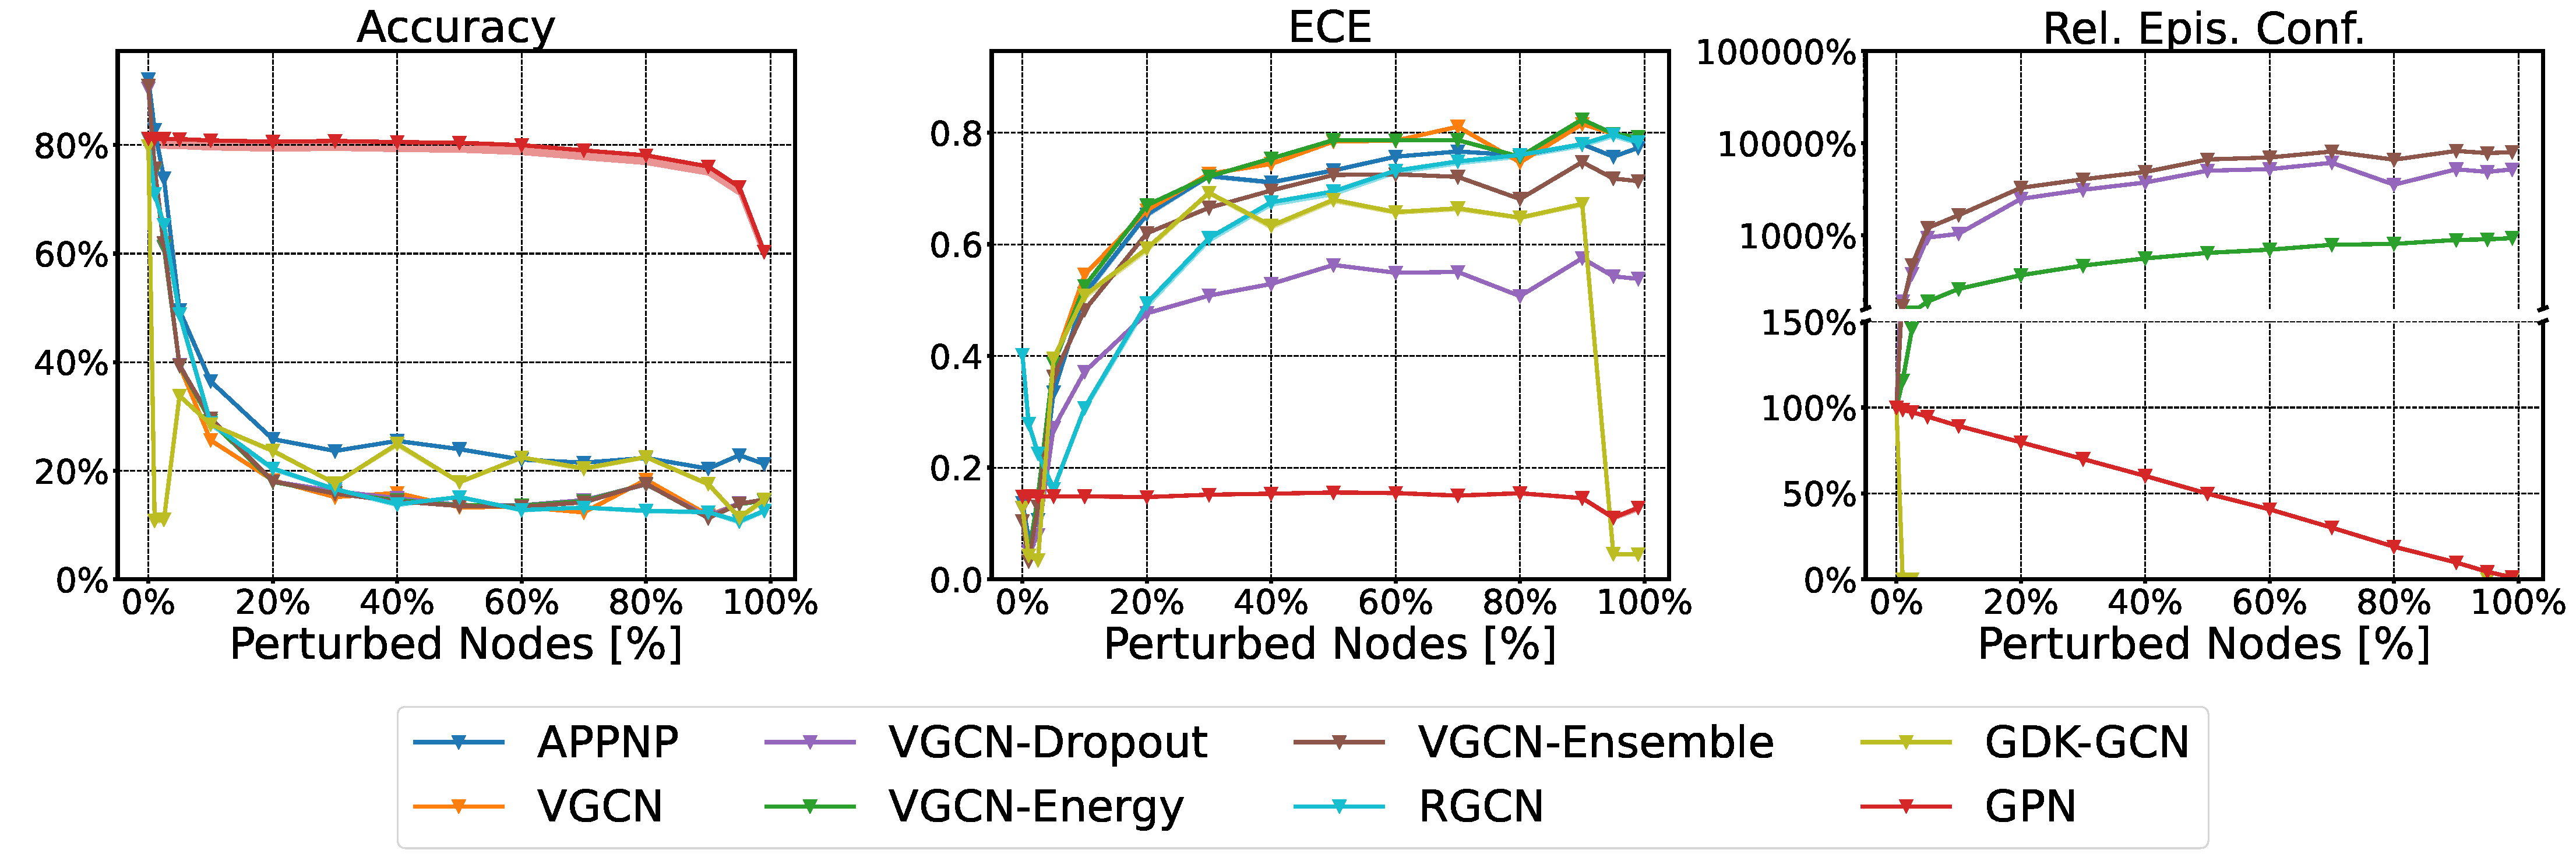
\includegraphics[width=\textwidth]{sections/009_neurips2021/resources/plots/AmazonPhotos-normal-shift.pdf}
        \caption{Unit Gaussian Feature Shift}
    \end{subfigure}
    \begin{subfigure}{\textwidth}
        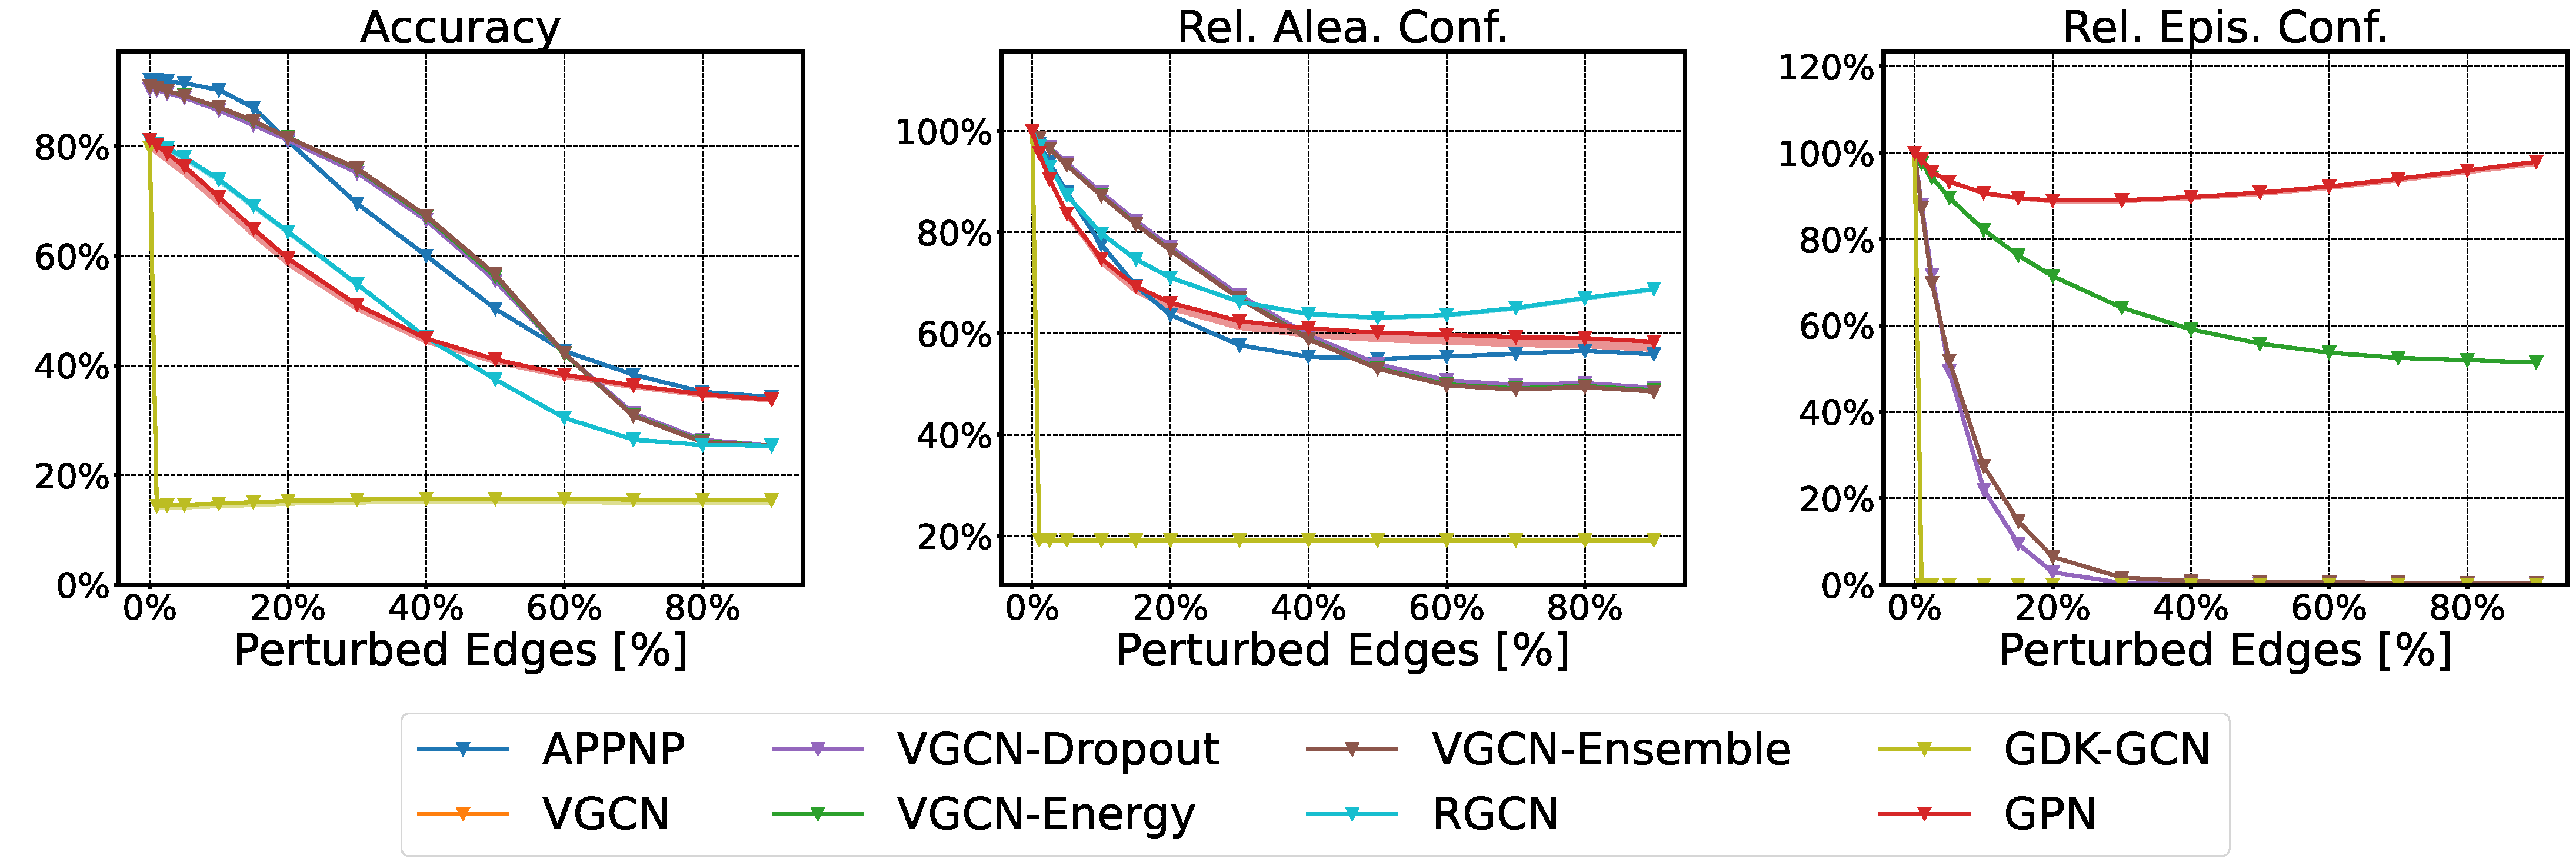
\includegraphics[width=\textwidth]{sections/009_neurips2021/resources/plots/AmazonPhotos-random-shift.pdf}
        \caption{Random Edge Shift}
    \end{subfigure}
    \begin{subfigure}{\textwidth}
        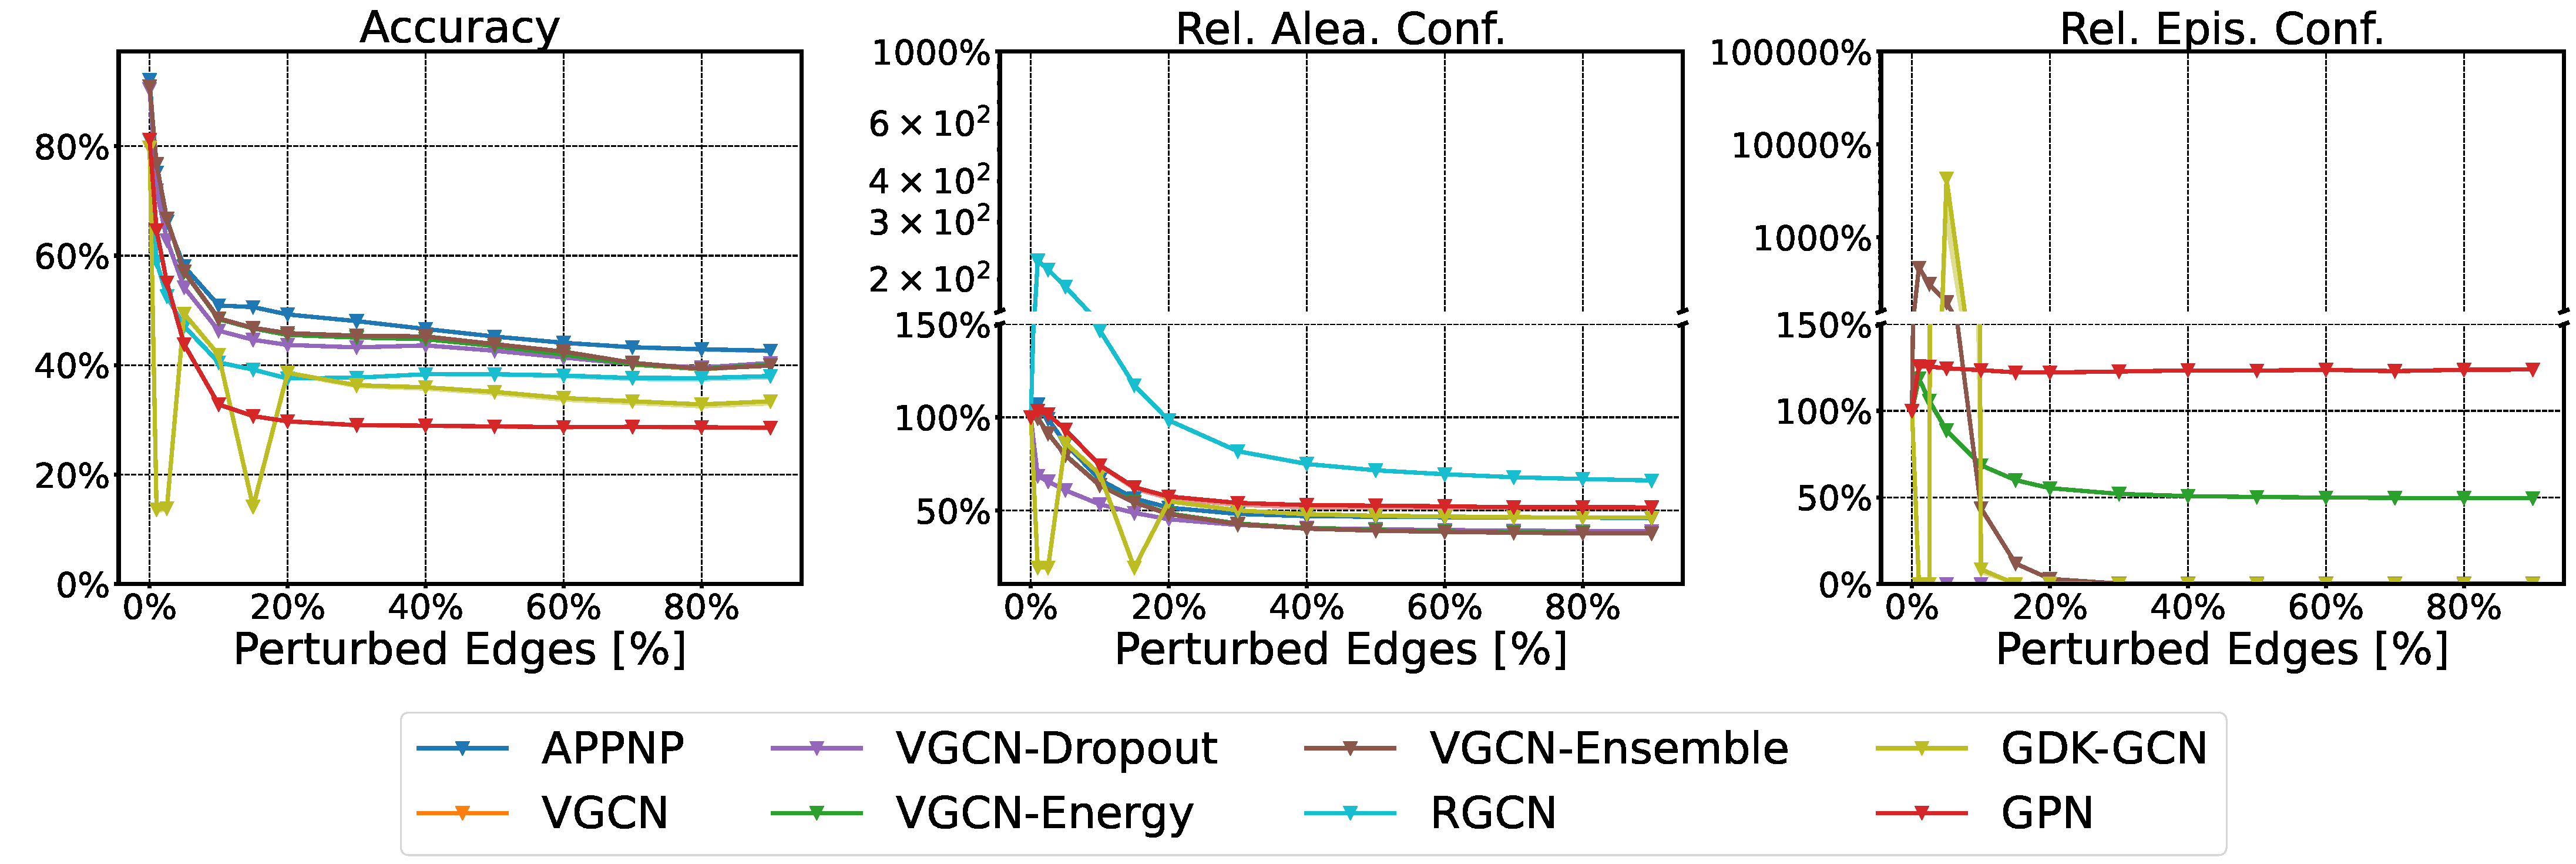
\includegraphics[width=\textwidth]{sections/009_neurips2021/resources/plots/AmazonPhotos-dice-shift.pdf}
        \caption{DICE \citep{Waniek2018} Edge Shift}
    \end{subfigure}
    \caption{Relative performance over different degrees of corruption of \emph{Amazon Photos}. For feature shifts, we perturb different fractions of nodes (whose features are replaced with either random vectors from a Bernoulli noise or a Unit Gaussian noise) and show accuracy, ECE, and relative average epistemic confidence. For edge shifts, we perturb different fractions of edges (by replacing them at random or using the global and untargeted DICE \citep{Waniek2018} attack) and show accuracy, relative average aleatoric confidence, and relative average epistemic confidence.}
    \label{fig:shift-amazon-photos}
\end{figure}